%
\documentclass{chi-ext}
% Please be sure that you have the dependencies (i.e., additional LaTeX packages) to compile this example.
% See http://personales.upv.es/luileito/chiext/

%% EXAMPLE BEGIN -- HOW TO OVERRIDE THE DEFAULT COPYRIGHT STRIP -- (July 22, 2013 - Paul Baumann)
\copyrightinfo{Copyright {2014} held by First Author. Rights Licensed to ACM}
%% EXAMPLE END -- HOW TO OVERRIDE THE DEFAULT COPYRIGHT STRIP -- (July 22, 2013 - Paul Baumann)

\title{Firmware: The Missing Blueprint}

% Notice how author names are alternately typesetted to appear ordered in 2-column format;
% i.e., the first 4 autors on the first column and the other 4 auhors on the second column.
% Actually, it's up to you to strictly adhere to this author notation.
\author{
  \alignauthor{
        \textbf{First Author}\\
        \affaddr{AuthorCo, Inc.}\\
        \affaddr{123 Author Ave.}\\
        \affaddr{Authortown, PA 54321 USA}\\
        \email{author1@anotherco.com}
  }
%  \alignauthor{
%        \textbf{Cefn Hoile}\\
%        \affaddr{Highwire DTC}\\
%        \affaddr{Lancaster University}\\
%        \email{c.hoile@lancaster.ac.uk}
%  }
  \vspace{2em}
  \begin{figure}
  \centering
  \includegraphics[width=260]{blueprint.jpg}
  \end{figure}
  \vspace{2em}
}

% Paper metadata (use plain text, for PDF inclusion and later re-using, if desired)
\def\plaintitle{CHI LaTeX Extended Abstracts Template}
\def\plainauthor{Luis A. Leiva}
\def\plainkeywords{Guides, instructions, author's kit, conference publications}
\def\plaingeneralterms{Documentation, Standardization}

\hypersetup{
  % Your metadata go here
  pdftitle={\plaintitle},
  pdfauthor={\plainauthor},  
  pdfkeywords={\plainkeywords},
  pdfsubject={\plaingeneralterms},
  % Quick access to color overriding:
  %citecolor=black,
  %linkcolor=black,
  %menucolor=black,
  %urlcolor=black,
}

\usepackage{verbatim}
\usepackage{graphicx}   % for EPS use the graphics package instead
\usepackage{balance}    % useful for balancing the last columns
\usepackage{bibspacing} % save vertical space in references
\renewcommand{\sfdefault}{phv} % Arial
\fontsize{8.5}{10}
\begin{document}

\marginpar{
\begin{figure}
  \begin{center}
  \includegraphics[width=\marginparwidth]{xmas.jpg}
  \caption{Flashing Tree Lights}
  \label{fig:marginparsample}
  \end{center}  
\end{figure}
\vspace{1em}
}

\marginpar{
\begin{figure}
  \begin{center}
  \includegraphics[width=\marginparwidth]{microwave.jpg}
  \caption{Domestic Microwave}
  \label{fig:marginparsample}
  \end{center}  
\end{figure}
\vspace{1em}
}

\marginpar{
\begin{figure}
  \begin{center}
  \includegraphics[width=\marginparwidth]{radio.jpg}
  \caption{Digital Radio}
  \label{fig:marginparsample}
  \end{center}  
\end{figure}
\vspace{1em}
}

\maketitle

\begin{abstract}
For a digitally-controlled product, its programmed behaviour, authored through firmware,  will heavily influence user experience. We contrast three caricatures of practice in  which product configurations are either \emph{discovered}, \emph{decided} or \emph{designed}, and focus on the role of  reflective practice, through sketching and boundary objects as a foundation for design. On this analysis, established practice in firmware engineering for selecting programmed behaviour does not satisfy the criteria for being reflectively designed. We examine what obstacles exist to applying reflective practices when selecting the \emph{behaviour} of products, and propose a programme to identify artefacts and processes which can facilitate this work.
\end{abstract}

\begin{comment}
\vspace{1mm}
\noindent
{\bf Categories and Subject Descriptors:} D.2.1 {Requirements/Specification}: {Elicitation Methods

\vspace{1mm}
\noindent
{\bf General Terms:} Enter your choices of the 16 terms.

\vspace{1mm}
\noindent
{\bf Keywords:} Enter your choices.
 \end{comment}

\keywords{Firmware, Microcontrollers, Product Design, Design Interactions, Sketching, Boundary Objects}

\category{D.2.1}{Requirements/Specifications}{Elicitation} 
 
\terms{Design, Human Factors, Experimentation

% =============================================================================
\section{Introduction}
% =============================================================================

An inclusive definition of design, offered by Feng and Feenberg [], is "a process of consciously shaping an artifact to adapt it to specific goals and environments". 

However, not all shaping practices adopt a designerly [] world-view. Some are close to a scientific method, where choices are \emph{discovered}, deducing them from facts. For example, a material's physical properties can eliminate it from consideration, or experiments can recommend employing a particular approach over an alternative. Other practices map a space of solutions on many dimensions of assessment, so a configuration can be \emph{decided} based on an explicit or implicit scheme of values and preferences [].

\marginpar{
\begin{figure}
  \begin{center}
  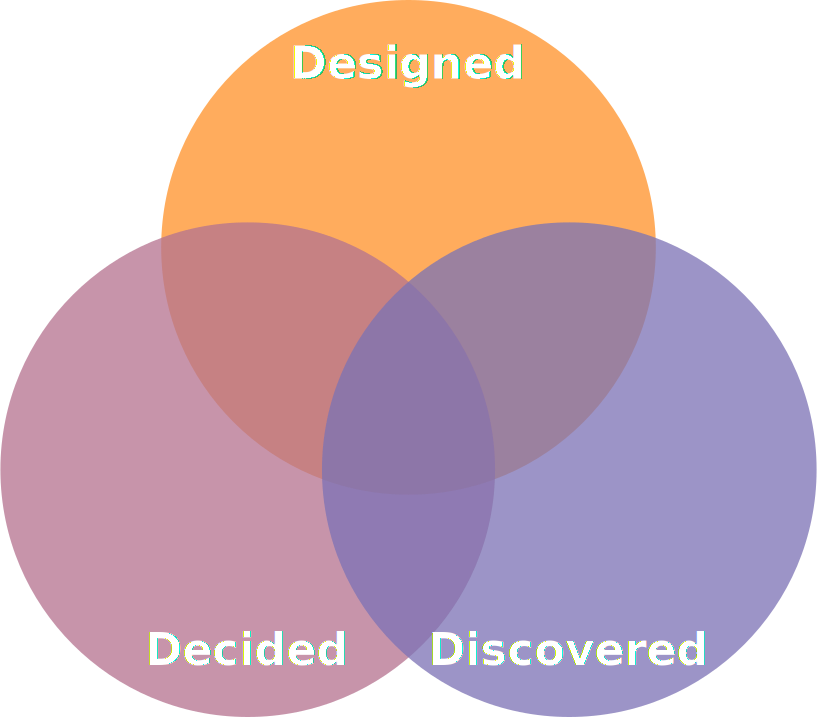
\includegraphics[width=\marginparwidth]{disciplines.jpg}
  \caption{Configuration Choice}
  \label{fig:marginparsample}
  \end{center}  
\end{figure}
}

So, how is designing distinct from discovering or decision-making? In this paper, we employ a definition of design, following Fallman[] and Louridas[], where the phrase \emph{designed} is reserved for artifact shaping which is arrived at through reflective processes [Schon]. \emph{Designed} preferences are neither \emph{discovered} through evidence gathering, nor \emph{decided} through systematic analysis of a space of configurations. Instead, a designer engages in a "conversation with materials" [Schon], a dynamic process in which "the materials [designers] use begin to 'talk back'". [Ozenc et al]

\marginpar{
\begin{figure}
  \begin{center}
  \includegraphics[width=\marginparwidth]{bikelight.jpg}
  \caption{Bikelights are computers too}
  \label{fig:marginparsample}
  \end{center}  
\end{figure}
}
Our position resonates strongly with Fallman's [], that sketching is "the archetypal activity of the design approach". However, if there are no candidate practices within firmware engineering which parallel \emph{sketching}, and if reflective techniques are central to value-creation in all design disciplines, we may ask whether product firmware is actually designed at all?

This paper explores candidate materials to support reflective design within firmware engineering, considering approaches used within the field and comparing them to those from established design disciplines. We offer reasons why familiar approaches cannot be trivially transferred to firmware engineering. We then propose a number of candidates for reflective materials which may be used effectively in firmware design and describe a programme of experimentation to discover how those tools and approaches may sustain the co-design of product firmware.

% =============================================================================
\section{Scope: Screenless Devices}
% =============================================================================

Our work focuses on simple products with no operating system, graphical interface, or application marketplace. These range from flashing fairy lights through domestic microwaves to digital radios. Selecting this domain excludes simplistic design approaches which treat rich interface design as an adequate proxy for interaction design, while leaving product behaviour underspecified.

Cateye's SL110 Loop Orbit bikelights illustrate how a product design process which facilitates user engagement and reflective exploration is sorely needed in this segment. A typical purchaser reports "The back light turns off after 1 minute! I can not use the set when cycling at night as it is unsafe."  A bike light unsuitable for use at night fails spectacularly to meet its design brief, yet the small print of the product manual reveals the secret -  "Deactivate...�Try Me�...mode (by pressing and holding the light for 30 seconds until it flashes quickly and shuts off)".

% =============================================================================
\section{Sketching, Immateriality, Processuality}
% =============================================================================

Design disciplines such as architecture have mature techniques to engage end-users early in the design process, whilst stimulating and recording multiple alternative choices for downstream implementation. These techniques range from unstructured, informal practices such as sketching, brainstorming, and low-fidelity prototypes through to more formal structured practices such as method cards or blueprints. They help �design intent� to be communicated, and facilitate reflection (Schon 1992). The techniques act to surface, record and resolve concerns in design choices before significant investments are made fabricating prototypes or materialising the final design.

\marginpar{
\begin{figure}
  \begin{center}
  \includegraphics[width=\marginparwidth]{architecture.jpg}
  \caption{Projective views such as blueprints support both reflection and collaboration}
  \label{fig:marginparsample}
  \end{center}  
\end{figure}
\vspace{1em}
}

Designers rely on sketching because it �supports cognition in ways that lead to creativity�, including �re-interpretive cycles of idea generation� \cite{Craft}. They "rough out ideas�, then �critique what they have done" \cite{Ozenc}.

Familiar techniques allow 2D graphical artifacts or 3D physical products to be represented on the page of a sketchbook and reflected upon. However, sketching the design of product \emph{firmware} presents problems, since it is both immaterial \cite{Ozenc} and processual \cite{Bratteteig}. Since it is immaterial there is no trivial 2D projection of its code which a non-programmer can be expected to author or interpret. Since it is processual, by nature determined by circumstance and history, static representations can deliver only a partial view of the product behaviour. As a result, when attempting to design interactive systems through sketching, designers feel they have "not had enough feedback to know if this is the design they want� \cite{Ozenc}.

% =============================================================================
\section{Architecture versus Firmware Engineering}
% =============================================================================

Many participants in a physical design process, such as the design of a building, lack the skills needed to actually materialise the product. Formal drawings such as blueprints capture implementation commitments, guiding and constraining a specialist production process, but can also act as a \emph{boundary object} \cite{Star}, catalysing knowledge exchange between a wide range of stakeholders, helping to integrate clients' experience of the market and users' experience of the domain in the design process.

Architects also pioneered the use of \emph{pattern languages} \cite{Alexander}both to describe a space of design possibilities, but just as importantly as a technique for brokering agreement with stakeholders about design alternatives.

Through blueprints and pattern languages, early engagement with an architectural design can take place without either building the design or demanding that collaborators have the skills needed to materialise the design. 

Although software engineering inherited the concept of \emph{patterns} from Alexander's architectural practice \cite{Gamma} the important intent,that patterns should sustain stakeholder engagement was lost in translation. The representations which characterise implementation are accessible principally to programmers \cite{Petre} - those skilled in materialising digital behaviours - and can not effectively catalyse knowledge exchange with others. By excluding key stakeholders until working systems are ready to be tested, this restricts the design contributions others can make. 

Firmware development begins with a requirements document, and proceeds through modelling constructs and program code until a single prototype implementation can be deployed [Ganssle 2000]. During these phases many choices are made which will impact on user experience. However, it is only after a working prototype is deployed that feedback is anticipated from non-programmers on the behaviour design choices already made [Punkka 2005, van der Helm 2008]. 
\marginpar{
\begin{figure}
  \begin{center}
  \includegraphics[width=\marginparwidth]{wizard_of_oz.jpg}
  \caption{The Wizard Of Oz}
  \label{fig:marginparsample}
  \end{center}  
\end{figure}
\vspace{2em}
}
\marginpar{
\begin{figure}
  \begin{center}
  \includegraphics[width=\marginparwidth]{scratch.png}
  \caption{A Scratch Program and its outcome.}
  \label{fig:marginparsample}
  \end{center}  
\end{figure}
}

This raises the concern that behaviour design decisions for digitally-controlled products could be made overwhelmingly by software engineers on behalf of users, exploring few alternatives, and in isolation from user design contributions (Norman 2006). Assuming that a prototype is needed to sustain engagement, user feedback is only possible late in the firmware design process and inherently centres around approving or critiquing a single behaviour design configuration. Critiques of firmware design [Norman 2002, 2010, Thimbleby 2007, Ganssle 2000) suggest that limitations of existing practice has a direct impact on the quality of products in the marketplace.

% =============================================================================
\section{Candidate Materials}
% =============================================================================

A promising technique for non-programmers to specify their intended behaviours in the context of a specific prototype and use context is the use of Wizard of Oz (WOZ) prototyping (Gould et al 1983)(Bernsen et al 1994)(Dow et al 2005), a practice inspired by the Wizard of Oz film, in which the character of the wizard turns out to be a man hiding behind a curtain, manipulating dramatic effects from a console. By avoiding upfront software engineering, WOZ prototyping �helps designers avoid getting locked into a particular design or from working under an incorrect set of assumptions about the users� preferred mode of interaction, because it enables design exploration and evaluation� and allows �evaluating partially complete systems� (Dow et al 2005)

WOZ bypasses the need to express behaviours as code, but this has both advantages and disadvantages. In the short term, it means there is little friction or delay between conceiving an idea and representing it to others in a workshop, but in the long term the potential lack of precision, and the potential for behaviours which are actually impossible for a computer to enact, could lead to issues during implementation unless these issues are caught early and eliminated.

MIT's Scratch programming environment enables ordinary users to construct simple event-driven programs by constructing sentences from natural language tiles whose label, color and shape provide important cognitive clues as to
their syntax and semantics. When complete, programs can be read as an english sentence, but also 

Scratch is intended as a pedagogical tool rather than an orchestration tool in its own right and is oriented towards the domain of multimedia-driven
applications.

We outline the preferred features by analogy with effective tools from other disciplines, and we detail a program of future co-design experimentation which we hope will allow us to explore and validate candidate representations.


% =============================================================================
\section{Conclusion}
% =============================================================================

Critiques levelled at mainstream interaction design suggest that practice should change.


Because of the choice of workshop participants, we have the benefit of users representing themselves as �expert of their experiences� (Visser et al 2005) and bringing intimate domain knowledge of the field. However, for users to fulfil this role effectively they must be offered �appropriate tools for expressing themselves� (Sanders and Stappers 2008).

and bricolage [Levi-Strauss], building on design theorist's claims that  [Fallman] and that "design in all its guises is a form of bricolage"[Louridas].

\section{Acknowledgements}
NYU Dead Media Archive [Blueprint image]
Creative Commons imagery [Flickr accounts clagnut,]
SarahMumOf3 for Xmas Light controller


\section{References format}
References must be the same font size as other body text.
% REFERENCES FORMAT
% References must be the same font size as other body text.

\balance
\bibliographystyle{acm-sigchi}
\bibliography{sample}

\end{document}
